%chapters/low-rate-cs-uwb-pos.tex
\subsection{Low Rate CS Pre-Mixing for UWB Positioning}
\begin{figure*}[!t]
\centering
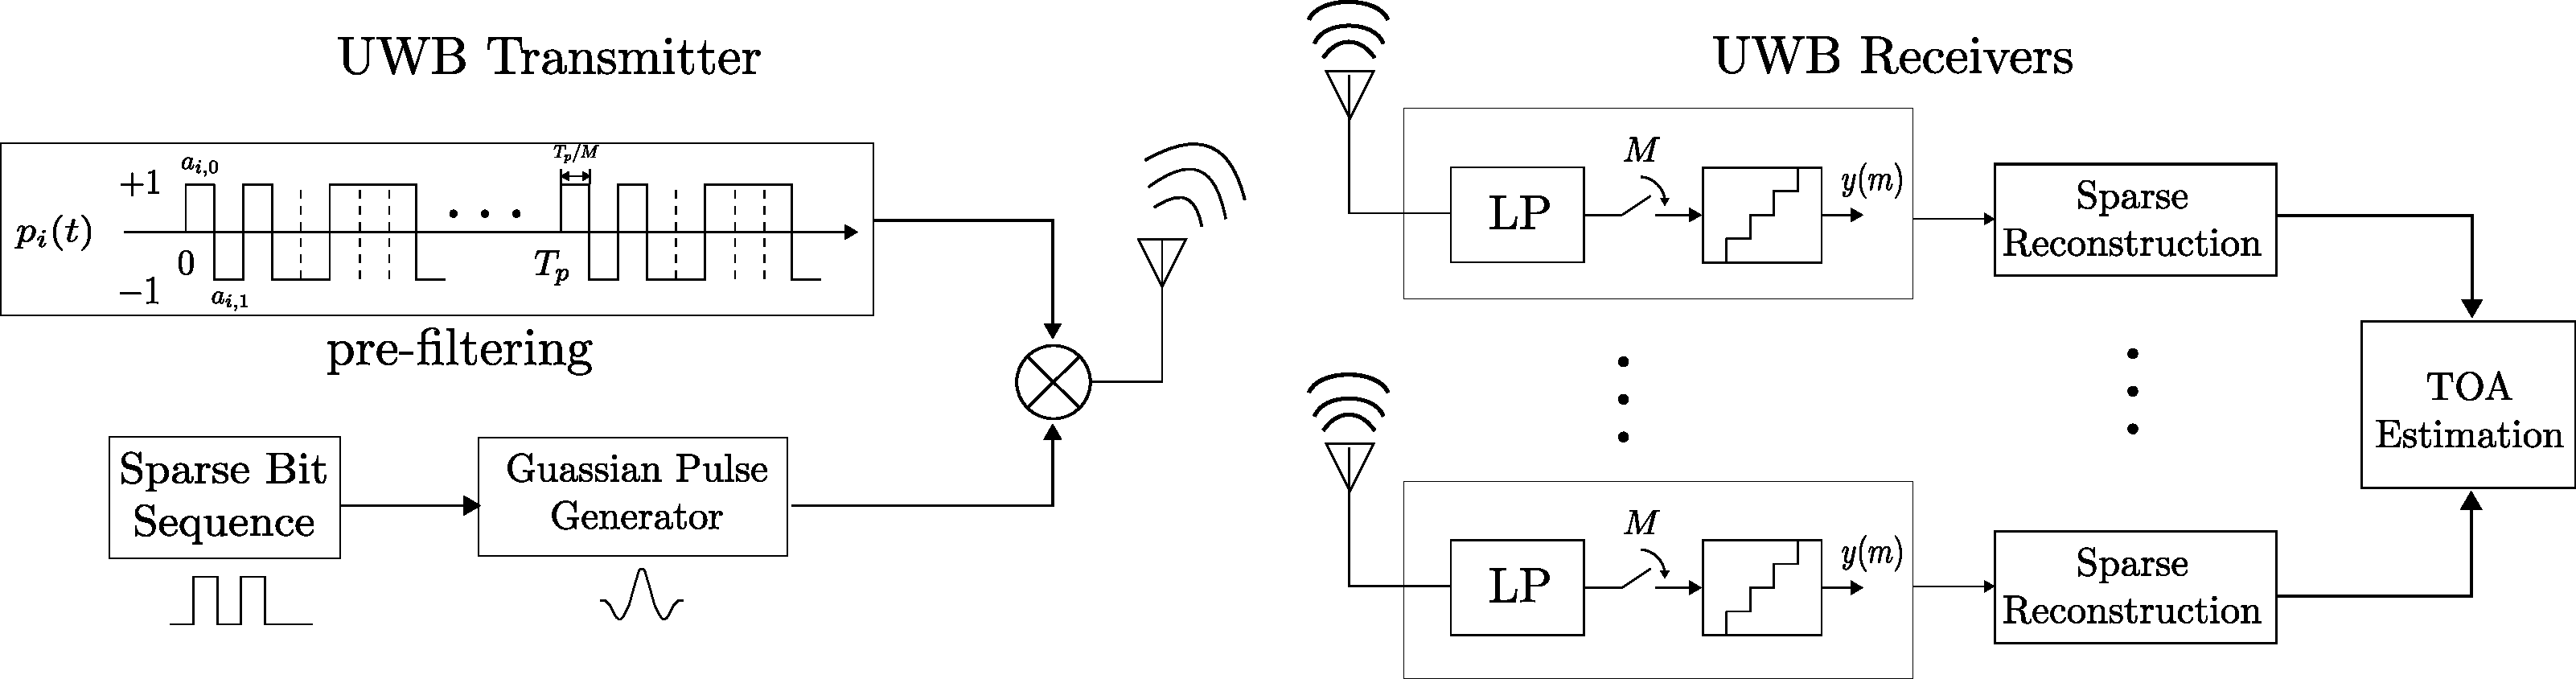
\includegraphics[width=6.0in]{cs-uwb-design2.pdf}
\DeclareGraphicsExtensions.
\caption{Block diagram of low-rate CS pre-filtering UWB positioning system.}
\label{cs-uwb-design2}
\end{figure*}

As mentioned, both CS receivers and CS transmitters suffer from high-data rate random projection operation, where the alternative rate of pseudo-random sequence is required (often equal or above 5 GHz in such cases). This requirement generates a heavy burden on bandwidth of hardware mixers and high frequency noise. 

In order to solve this problem but meanwhile preserve the energy efficient feature in CS transmitters, this paper propose an low-rate CS pre-mixing (LRCSPM) UWB positioning system shown in Fig.\ref{cs-uwb-design2}: At the transmitter side, the new system provides a relatively low-rate pseudo-random sequence to mix the generated Gaussian pulses. At the receivers side, it sacrifices the compression ratio (or sampling rate) to catch up with the equivalent performance as that in the CS receivers based UWB system. As a result, the trade-off between the random projection rate and the sub-Nyquist sampling rate offers a more energetic balanced system, where no hardware devices suffers from the limitation brought from the high data rate sequence. In addition, the positioning accuracy is successfully improved compared to the original UWB system. 

\subsection{System Model}

Based on the IR-UWB indoor positioning system model in (\ref{eq_recv}), the new structure of our system can be regarded as shown in Fig.\ref{cs-uwb-design2}. At the transmitter, the a pseudo-random sequence (PRS) whose variables are chosen from ${-1,+1}$ are generated using a relatively low sub-Nyquist alternative rate. When a UWB pulse generated, first it will be randomly mixed by the pseudo-random sequence, and then broadcasted to indoor environment from the transmitter. Afterwards, receivers directly downsample the signals at a relatively low rate. Finally, after processing the sparse reconstruction (i.e OMP or BP), the original TOA based algorithm can work for indoor positioning. In addition, these steps at receivers can be executed pipelined as \cite{yang2011compressive}. Hence, based on the workflow of the new architecture, the math model of this sytem can be represented as following matrix form (\ref{eq_sys_m}):
\begin{equation}
\label{eq_sys_m}
y = D * H * P * x
\end{equation}
where $y$ are discrete sampled observations from low rate ADCs at receivers, and $x$ is the generated UWB Gaussian pulses at traditional transmitters. Here $H$ is the correspondingly Toeplitz matrix which presents the signal convolution using IEEE 802.15.4a model in (\ref{eq_chan}), and $F$ stands for the random projetion step, which is a diagnose matrix whose variables are randomly chosen from $\{-1,+1\}$ but alternatives at a sub-Nyquist low rate. The $D$ represents the downsampling behavior. It is a $m\times N$ matrix ($m << N$) with 0-1 entries , and each of its rows contains a block of $\frac{m}/{N}$ contiguous ones, which has been used for simulation in \cite{tropp2010beyond}. Then $\hat x$ can be reconstructed from various sparse reconstruction algorithm such as BP, OMP and CoSaMP. At last, the recovered signal $\hat x$ is applied for TOA based positioning estimation.
